\documentclass[letterpaper, onecolumn,10pt]{IEEEtran}

\usepackage{graphicx}
\usepackage{amssymb}
\usepackage{amsmath}
\usepackage{amsthm}

\usepackage{alltt}
\usepackage{float}
\usepackage{color}
\usepackage{url}
\usepackage{listings}
\usepackage{ifthen}


\usepackage[TABBOTCAP, tight]{}

\usepackage{geometry}
\geometry{textheight=8.5in, textwidth=6in}

%random comment

\newcommand{\cred}[1]{{\color{red}#1}}
\newcommand{\cblue}[1]{{\color{blue}#1}}

\usepackage{hyperref}
\usepackage{geometry}
\usepackage{caption}
\usepackage{url}
\usepackage{natbib}

\begin{document}
    \begin{titlepage}
    \newcommand{\HRule}{\rule{\linewidth}{0.5mm}}
    \center
    \textsc{\Large Oregon State University}\\[1.5cm]
    \textsc{\Large ST 314}\\[0.5cm]
    \textsc{\Large Summer 2019}\\[0.5cm]
    \HRule \\[0.4cm]
    { \huge \bfseries Data Analysis Six}\\[0.4cm] % Title of your document
    \HRule \\[1.5cm]
    \begin{minipage}{0.4\textwidth}
        \begin{flushleft} \large
        \emph{Author:}\\
        Thomas Noelcke
        \end{flushleft}
    \end{minipage}
    \begin{minipage}{0.4\textwidth}
        \begin{flushright} \large
        \emph{Instructor:} \\
        Katie Jager\\
        \end{flushright}
    \end{minipage}\\[2cm]
		\end{titlepage}
        
        \section{Part 1}
            \subsection{}
             %include graphics here side by side box plot
             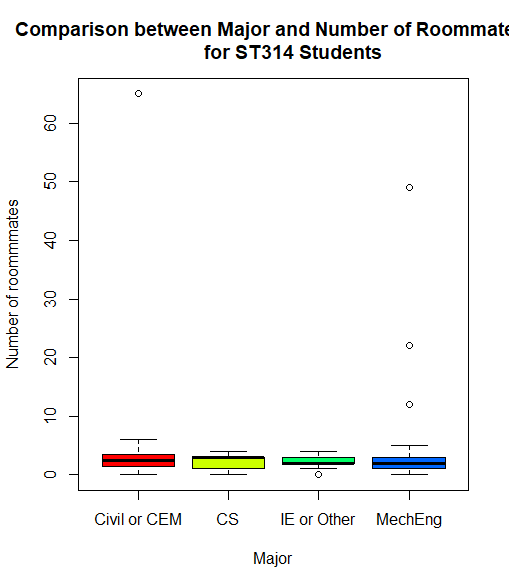
\includegraphics[]{week6/images/Rplot.png}
             
             \subsection{}
             Based on the side by side box plots it does appear that there are differences in the average. It appears that CS has a higher average in comparison to the other majors. The other majors seem to have similar averages. However, Mechanical and Civil both have outliers.\\
		
		    \subsection{}
		    The null hypothesis and alternative hypothesis are shown below:
            \[
                H_0 = \mu_{civilandCEM} = \mu_{cs} = \mu_{IE} = \mu_{mech}
            \]
            \[
                H_a =
            \]
            Two or more are different
            
            \subsection{}
            The conditions for this set of sample data is not ideal. This sample is not completely random as this sample is selected from students that are in ST314. Additionally, all of the students in this class are taking the online version of the class. It is also fair to note that the standard deviations for the different samples vary widely with IE or other at 1.043 on the low end and Civil or CEM on the high end with 11.926.\\
            
            \subsection{}
            \begin{lstlisting}
            Df Sum Sq Mean Sq F value Pr(>F)
Major         3    108   36.07   0.742  0.529
Residuals   136   6613   48.63   
            \end{lstlisting}
            
            From the table above we can say that the MSTr is 36.07 and the MSE is 48.63.\\ 
            
            \subsection{}
                \subsubsection{}
                We cannot say that there is significant difference between at least two of the populations. With a P-Value of 0.539 and an F value of 0.742.\\
                
                \subsubsection{}
                There is not significant evidence to reject the null hypothesis that the different majors have different population means in terms of number of room mates.\\
            \subsection{}
                \subsubsection{}
                    \begin{lstlisting}
                            diff       lwr      upr     p adj
CS-Civil or CEM          -2.328571 -6.418790 1.761647 0.5537141
IE or Other-Civil or CEM -2.476190 -7.349825 2.397444 0.6433715
MechEng-Civil or CEM     -1.202179 -4.904243 2.499885 0.8759930
IE or Other-CS           -0.147619 -4.826661 4.531423 0.9998599
MechEng-CS                1.126392 -2.315468 4.568252 0.8734787
MechEng-IE or Other       1.274011 -3.069814 5.617837 0.9050928
                    \end{lstlisting}
                
                \subsubsection{}
                In this case all of the comparisons are significant in that they all pass the P-Value test.\\
                
                \subsubsection{}
                    The difference with the smallest P value is the comparison between CS and Civil and CEM. This statistic shows that the difference between CS and Civil/CEM in terms of number of room mates will be between -6.41 and 1.761 room mates.\\
        \section{Part 2}
            \subsection{}
            From the bar chart we can say that 90.9 percent of students have a social networking profile.\\
            \subsection{}
            It may be reasonable to assume that this data represents the entire engineer collage data because at 132 students is considered large. This means that the chance that this sample is an outlier is low as the standard deviation will also be low or as shown below:
            
            \[
                \sqrt{\dfrac{p(1-p)}{n}}
            \]
            
            It's also fair to say that ST314 captures a pretty good random sample of the college of engineering as we all have to take this class and the prerequisites are typically taken early for most students.\\
            
            \subsection{}
            This sample could also be skewed because we are all online students in this class. This means we are all already participating in some sort of online activity and are likely to have social media profiles as well.\\
            
            \subsection{}
            shown below is my check for the conditions of the sample size:
            
            \[
                n x p_0 \geq 10 and n x(1-p_0) \geq 10
            \]
            \[
                = 132*0.909 \geq 10 and 132 *(1-0.09) \geq 10
            \]
            \[
                = 119.988 \geq 10 and  12.012 \geq 10
            \]
            
            Conditions are acceptable.
            
            \subsection{}
            Shown below is my estimate of a 95\% confidence interval for students in the COE with a social media profile.
            
            \[
                p_hat \pm z^* \sqrt{\dfrac{p_hat(p_hat - 1)}{n}}
            \]
            \[
                = 0.909 \pm 1.96 \sqrt{\dfrac{0.909(1 - 0.909)}{132}} = [0.860, 0.958]
            \]
            
            \subsection{}
            There is a 95 percent chance that the true proportion of students in the COE that have a social media profile is between 0.860 and 0.958 with a point estimate of 0.909.\\
            
		\end{document}